\section{Multsiplit and Common Approaches}\label{sec:init_approaches}
In this section, we first formally define the multisplit as a primitive algorithm.
Next, we describe some common approaches for performing the multisplit algorithm, which form a baseline for the comparison to our own methods, which we then describe in Section~\ref{sec:algorithm}.

\subsection{The multisplit primitive}\label{sec:multisplit}

We informally characterize multisplit as follows:

\begin{itemize}
\item Input: An unordered set of keys or key-value pairs. ``Values'' that are larger than the size of a pointer use a pointer to the value in place of the actual value.
\item Input: A function, specified by the programmer, that inputs a key and outputs the bucket corresponding to that key (\emph{bucket identifier}).
For example, this function might classify a key into a particular numerical range, or divide keys into prime or composite buckets.
\item Output: Keys or key-value pairs separated into $m$ buckets. Items within each output bucket must be contiguous but are otherwise unordered. Some applications may prefer output order within a bucket that preserves input order; we call these multisplit implementations ``stable''.
% \item $m$, the number of buckets: a modest number, say more than 2 but less than or equal to 64. For two buckets, split is traditionally the best solution, and as the number of buckets grows, the multisplit problem converges to a full sort.
\end{itemize}

\noindent
More formally, let $\mathbf{u}$ and $\mathbf{v}$ be vectors of $n$ \emph{key} and \emph{value} elements, respectively.
Altogether $m$ buckets $B_0, B_1, \dots, B_{m-1}$  partition the entire key domain such that each key element uniquely belongs to one and only one bucket.
Let $\defn{f}(\cdot)$ be an arbitrary bucket identifier that assigns a bucket ID to each input key (e.g., $\defn{f}(u_i) = j$ if and only if $u_i \in B_j$).
Throughout this paper, $m$ always refers to the total number of buckets.
For any input key vector, we define \emph{multisplit} as a permutation of that input vector into an output vector. The output vector is densely packed and has two properties: (1) All output elements within the same bucket are stored contiguously in the output vector, and (2) All output elements are stored contiguously in a vector in ascending order by their bucket IDs\@. Optionally, the beginning index of each bucket in the output vector can also be stored in an array of size $m$.
Our main focus in this paper is on 32-bit keys and values (of any data type).

This multisplit definition allows for a variety of implementations. It places no restrictions on the order of elements within each bucket before and after the multisplit (intra-bucket orders); buckets with larger indices do not necessarily have larger elements. In fact, key elements may not even be comparable entities, e.g., keys can be strings of names with buckets assigned to male names, female names, etc. We do require that buckets are assigned to consecutive IDs and will produce buckets ordered in this way.
Figure~\ref{fig:multisplit_example} illustrates some multisplit examples.
% We categorize multisplit problems into two cases of trivial and non-trivial bucket identifications.
% The former happens when the bucket identifier is an identity function and all keys are in $\{0,1,\dots, m-1\}$ and also equal to their bucket IDs (e.g., $\defn{f}(u_i) = u_i = j$ if and only if $u_i \in B_j$). In this case, a regular sort on keys (or key-values) is equivalent to a multisplit.
% Our main focus in this paper is on non-trivial cases, but we will consider trivial multisplits and possibility of using them for building our own radix sort in {\color{red} Section~\ref{}}.
Next, we consider some common approaches for dealing with non-trivial multisplit problems.

\begin{figure}
  \centering
  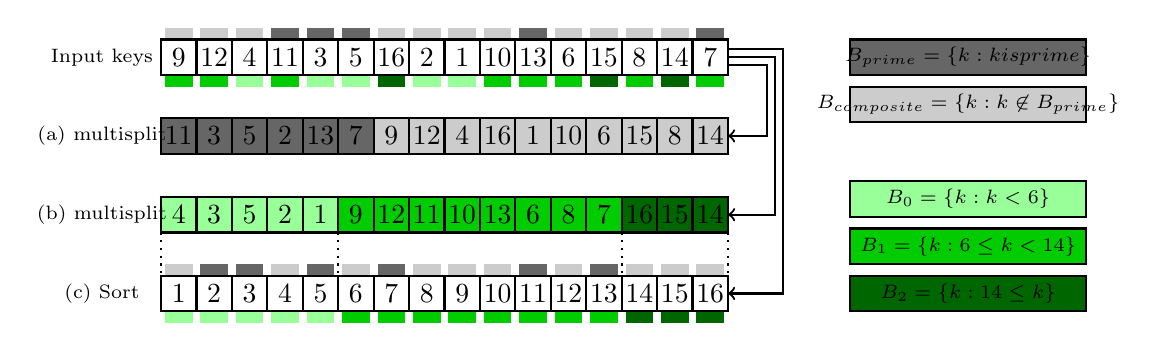
\begin{tikzpicture}
\def\recX{0.45}
\def\recY{0.45}
\def\idx{1}
\def\dx{0.45}
\def\deltaY{1.0}
\def\offsetX{-1.0}
\def\sortedKeys{{1,2,3,4,5,6,7,8,9,10,11,12,13,14,15,16}}
\def\inputKeys{{9, 12, 4, 11, 3, 5, 16, 2, 1, 10, 13, 6, 15, 8, 14, 7}}
\def\primeKeys{{11, 3, 5, 2, 13, 7, 9, 12, 4, 16, 1, 10, 6, 15, 8, 14}}
\def\multisplitKeys{{4, 3, 5, 2, 1, 9, 12, 11, 10, 13, 6, 8, 7, 16, 15, 14}} 
% \definecolor{dkblue}{rgb} {0.00,0.33,0.68}


\fill [white!80!black] (\offsetX + 0 * \dx + 0.05, 0.15) rectangle (\offsetX + 0 * \dx + \recX - 0.05, \recY + 0.15);
\fill [white!80!black] (\offsetX + 1 * \dx + 0.05, 0.15) rectangle (\offsetX + 1 * \dx + \recX - 0.05, \recY + 0.15);
\fill [white!80!black] (\offsetX + 2 * \dx + 0.05, 0.15) rectangle (\offsetX + 2 * \dx + \recX - 0.05, \recY + 0.15);
\fill [white!40!black] (\offsetX + 3 * \dx + 0.05, 0.15) rectangle (\offsetX + 3 * \dx + \recX - 0.05, \recY + 0.15);
\fill [white!40!black] (\offsetX + 4 * \dx + 0.05, 0.15) rectangle (\offsetX + 4 * \dx + \recX - 0.05, \recY + 0.15);
\fill [white!40!black] (\offsetX + 5 * \dx + 0.05, 0.15) rectangle (\offsetX + 5 * \dx + \recX - 0.05, \recY + 0.15);
\fill [white!80!black] (\offsetX + 6 * \dx + 0.05, 0.15) rectangle (\offsetX + 6 * \dx + \recX - 0.05, \recY + 0.15);
\fill [white!80!black] (\offsetX + 7 * \dx + 0.05, 0.15) rectangle (\offsetX + 7 * \dx + \recX - 0.05, \recY + 0.15);
\fill [white!80!black] (\offsetX + 8 * \dx + 0.05, 0.15) rectangle (\offsetX + 8 * \dx + \recX - 0.05, \recY + 0.15);
\fill [white!80!black] (\offsetX + 9 * \dx + 0.05, 0.15) rectangle (\offsetX + 9 * \dx + \recX - 0.05, \recY + 0.15);
\fill [white!40!black] (\offsetX + 10 * \dx + 0.05, 0.15) rectangle (\offsetX + 10 * \dx + \recX - 0.05, \recY + 0.15);
\fill [white!80!black] (\offsetX + 11 * \dx + 0.05, 0.15) rectangle (\offsetX + 11 * \dx + \recX - 0.05, \recY + 0.15);
\fill [white!80!black] (\offsetX + 12 * \dx + 0.05, 0.15) rectangle (\offsetX + 12 * \dx + \recX - 0.05, \recY + 0.15);
\fill [white!80!black] (\offsetX + 13 * \dx + 0.05, 0.15) rectangle (\offsetX + 13 * \dx + \recX - 0.05, \recY + 0.15);
\fill [white!80!black] (\offsetX + 14 * \dx + 0.05, 0.15) rectangle (\offsetX + 14 * \dx + \recX - 0.05, \recY + 0.15);
\fill [white!40!black] (\offsetX + 15 * \dx + 0.05, 0.15) rectangle (\offsetX + 15 * \dx + \recX - 0.05, \recY + 0.15);

\fill [black!20!green] (\offsetX + 0 * \dx + 0.05, -0.15) rectangle (\offsetX + 0 * \dx + \recX - 0.05, \recY - 0.15);
\fill [black!20!green] (\offsetX + 1 * \dx + 0.05, -0.15) rectangle (\offsetX + 1 * \dx + \recX - 0.05, \recY +-0.15);
\fill [green!40!white] (\offsetX + 2 * \dx + 0.05, -0.15) rectangle (\offsetX + 2 * \dx + \recX - 0.05, \recY - 0.15);
\fill [black!20!green] (\offsetX + 3 * \dx + 0.05, -0.15) rectangle (\offsetX + 3 * \dx + \recX - 0.05, \recY - 0.15);
\fill [green!40!white] (\offsetX + 4 * \dx + 0.05, -0.15) rectangle (\offsetX + 4 * \dx + \recX - 0.05, \recY - 0.15);
\fill [green!40!white] (\offsetX + 5 * \dx + 0.05, -0.15) rectangle (\offsetX + 5 * \dx + \recX - 0.05, \recY - 0.15);
\fill [black!60!green] (\offsetX + 6 * \dx + 0.05, -0.15) rectangle (\offsetX + 6 * \dx + \recX - 0.05, \recY - 0.15);
\fill [green!40!white] (\offsetX + 7 * \dx + 0.05, -0.15) rectangle (\offsetX + 7 * \dx + \recX - 0.05, \recY - 0.15);
\fill [green!40!white] (\offsetX + 8 * \dx + 0.05, -0.15) rectangle (\offsetX + 8 * \dx + \recX - 0.05, \recY - 0.15);
\fill [black!20!green] (\offsetX + 9 * \dx + 0.05, -0.15) rectangle (\offsetX + 9 * \dx + \recX - 0.05, \recY - 0.15);
\fill [black!20!green] (\offsetX + 10 * \dx + 0.05,- 0.15) rectangle (\offsetX + 10 * \dx + \recX - 0.05, \recY - 0.15);
\fill [black!20!green] (\offsetX + 11 * \dx + 0.05,- 0.15) rectangle (\offsetX + 11 * \dx + \recX - 0.05, \recY - 0.15);
\fill [black!60!green] (\offsetX + 12 * \dx + 0.05,- 0.15) rectangle (\offsetX + 12 * \dx + \recX - 0.05, \recY - 0.15);
\fill [black!20!green] (\offsetX + 13 * \dx + 0.05,- 0.15) rectangle (\offsetX + 13 * \dx + \recX - 0.05, \recY - 0.15);
\fill [black!60!green] (\offsetX + 14 * \dx + 0.05,- 0.15) rectangle (\offsetX + 14 * \dx + \recX - 0.05, \recY - 0.15);
\fill [black!20!green] (\offsetX + 15 * \dx + 0.05,- 0.15) rectangle (\offsetX + 15 * \dx + \recX - 0.05, \recY - 0.15);

\foreach \x in {0,...,15}
	\fill [white] (\offsetX + \x * \dx,0 * \recY) rectangle (\offsetX + \x * \dx + \recX, 0 * \recY + \recY);

\foreach \x in {0,...,15}
	\draw [black, thick] (\offsetX + \x * \dx,0 * \recY) rectangle (\offsetX + \x * \dx + \recX, 0 * \recY + \recY) node[pos=0.5]{\pgfmathparse{\inputKeys[\x]}\pgfmathresult} ;
\draw [] (-1.75,\recY/2) node{\scriptsize {Input keys}};
%%%

\foreach \x in {0,...,5}
	\fill [white!40!black] (\offsetX + \x * \dx,0 * \recY - \deltaY) rectangle (\offsetX + \x * \dx + \recX, 0 * \recY + \recY - \deltaY);

\foreach \x in {6,...,15}
	\fill [white!80!black] (\offsetX + \x * \dx,0 * \recY - \deltaY) rectangle (\offsetX + \x * \dx + \recX, 0 * \recY + \recY - \deltaY);	 

\foreach \x in {0,...,15}
	\draw [black, thick] (\offsetX + \x * \dx,0 * \recY - \deltaY) rectangle (\offsetX + \x * \dx + \recX, 0 * \recY + \recY - \deltaY) node[pos=0.5]{\pgfmathparse{\primeKeys[\x]}\pgfmathresult};

\draw [] (-1.75,\recY/2 - \deltaY) node{\scriptsize {(a) multisplit}};
%%%

\foreach \x in {0,...,4}
	\fill [green!40!white] (\offsetX + \x * \dx,0 * \recY - 2*\deltaY) rectangle (\offsetX + \x * \dx + \recX, 0 * \recY + \recY - 2*\deltaY);	 

\foreach \x in {5,...,12}
	\fill [black!20!green] (\offsetX + \x * \dx,0 * \recY - 2*\deltaY) rectangle (\offsetX + \x * \dx + \recX, 0 * \recY + \recY - 2*\deltaY);	 

\foreach \x in {13,...,15}
	\fill [black!60!green] (\offsetX + \x * \dx,0 * \recY - 2*\deltaY) rectangle (\offsetX + \x * \dx + \recX, 0 * \recY + \recY - 2*\deltaY);	 

\foreach \x in {0,...,15}
	\draw [black, thick] (\offsetX + \x * \dx,0 * \recY - 2*\deltaY) rectangle (\offsetX + \x * \dx + \recX, 0 * \recY + \recY - 2*\deltaY) node[pos=0.5]{\pgfmathparse{\multisplitKeys[\x]}\pgfmathresult};

\draw [] (-1.75,\recY/2 - 2*\deltaY) node{\scriptsize{(b) multisplit}};

%%%
\fill [white!80!black] (\offsetX + 0 * \dx + 0.05, 0.15- 3*\deltaY) rectangle (\offsetX + 0 * \dx + \recX - 0.05, \recY + 0.15- 3*\deltaY);
\fill [white!40!black] (\offsetX + 1 * \dx + 0.05, 0.15- 3*\deltaY) rectangle (\offsetX + 1 * \dx + \recX - 0.05, \recY + 0.15- 3*\deltaY);
\fill [white!40!black] (\offsetX + 2 * \dx + 0.05, 0.15- 3*\deltaY) rectangle (\offsetX + 2 * \dx + \recX - 0.05, \recY + 0.15- 3*\deltaY);
\fill [white!80!black] (\offsetX + 3 * \dx + 0.05, 0.15- 3*\deltaY) rectangle (\offsetX + 3 * \dx + \recX - 0.05, \recY + 0.15- 3*\deltaY);
\fill [white!40!black] (\offsetX + 4 * \dx + 0.05, 0.15- 3*\deltaY) rectangle (\offsetX + 4 * \dx + \recX - 0.05, \recY + 0.15- 3*\deltaY);
\fill [white!80!black] (\offsetX + 5 * \dx + 0.05, 0.15- 3*\deltaY) rectangle (\offsetX + 5 * \dx + \recX - 0.05, \recY + 0.15- 3*\deltaY);
\fill [white!40!black] (\offsetX + 6 * \dx + 0.05, 0.15- 3*\deltaY) rectangle (\offsetX + 6 * \dx + \recX - 0.05, \recY + 0.15- 3*\deltaY);
\fill [white!80!black] (\offsetX + 7 * \dx + 0.05, 0.15- 3*\deltaY) rectangle (\offsetX + 7 * \dx + \recX - 0.05, \recY + 0.15- 3*\deltaY);
\fill [white!80!black] (\offsetX + 8 * \dx + 0.05, 0.15- 3*\deltaY) rectangle (\offsetX + 8 * \dx + \recX - 0.05, \recY + 0.15- 3*\deltaY);
\fill [white!80!black] (\offsetX + 9 * \dx + 0.05, 0.15- 3*\deltaY) rectangle (\offsetX + 9 * \dx + \recX - 0.05, \recY + 0.15- 3*\deltaY);
\fill [white!40!black] (\offsetX + 10 * \dx + 0.05, 0.15- 3*\deltaY) rectangle (\offsetX + 10 * \dx + \recX - 0.05, \recY + 0.15- 3*\deltaY);
\fill [white!80!black] (\offsetX + 11 * \dx + 0.05, 0.15- 3*\deltaY) rectangle (\offsetX + 11 * \dx + \recX - 0.05, \recY + 0.15- 3*\deltaY);
\fill [white!40!black] (\offsetX + 12 * \dx + 0.05, 0.15- 3*\deltaY) rectangle (\offsetX + 12 * \dx + \recX - 0.05, \recY + 0.15- 3*\deltaY);
\fill [white!80!black] (\offsetX + 13 * \dx + 0.05, 0.15- 3*\deltaY) rectangle (\offsetX + 13 * \dx + \recX - 0.05, \recY + 0.15- 3*\deltaY);
\fill [white!80!black] (\offsetX + 14 * \dx + 0.05, 0.15- 3*\deltaY) rectangle (\offsetX + 14 * \dx + \recX - 0.05, \recY + 0.15- 3*\deltaY);
\fill [white!80!black] (\offsetX + 15 * \dx + 0.05, 0.15- 3*\deltaY) rectangle (\offsetX + 15 * \dx + \recX - 0.05, \recY + 0.15- 3*\deltaY);

\fill [green!40!white] (\offsetX + 0 * \dx + 0.05, -0.15- 3*\deltaY) rectangle (\offsetX + 0 * \dx + \recX - 0.05, \recY - 0.15- 3*\deltaY);
\fill [green!40!white] (\offsetX + 1 * \dx + 0.05, -0.15- 3*\deltaY) rectangle (\offsetX + 1 * \dx + \recX - 0.05, \recY +-0.15- 3*\deltaY);
\fill [green!40!white] (\offsetX + 2 * \dx + 0.05, -0.15- 3*\deltaY) rectangle (\offsetX + 2 * \dx + \recX - 0.05, \recY - 0.15- 3*\deltaY);
\fill [green!40!white] (\offsetX + 3 * \dx + 0.05, -0.15- 3*\deltaY) rectangle (\offsetX + 3 * \dx + \recX - 0.05, \recY - 0.15- 3*\deltaY);
\fill [green!40!white] (\offsetX + 4 * \dx + 0.05, -0.15- 3*\deltaY) rectangle (\offsetX + 4 * \dx + \recX - 0.05, \recY - 0.15- 3*\deltaY);
\fill [black!20!green] (\offsetX + 5 * \dx + 0.05, -0.15- 3*\deltaY) rectangle (\offsetX + 5 * \dx + \recX - 0.05, \recY - 0.15- 3*\deltaY);
\fill [black!20!green] (\offsetX + 6 * \dx + 0.05, -0.15- 3*\deltaY) rectangle (\offsetX + 6 * \dx + \recX - 0.05, \recY - 0.15- 3*\deltaY);
\fill [black!20!green] (\offsetX + 7 * \dx + 0.05, -0.15- 3*\deltaY) rectangle (\offsetX + 7 * \dx + \recX - 0.05, \recY - 0.15- 3*\deltaY);
\fill [black!20!green] (\offsetX + 8 * \dx + 0.05, -0.15- 3*\deltaY) rectangle (\offsetX + 8 * \dx + \recX - 0.05, \recY - 0.15- 3*\deltaY);
\fill [black!20!green] (\offsetX + 9 * \dx + 0.05, -0.15- 3*\deltaY) rectangle (\offsetX + 9 * \dx + \recX - 0.05, \recY - 0.15- 3*\deltaY);
\fill [black!20!green] (\offsetX + 10 * \dx + 0.05,- 0.15- 3*\deltaY) rectangle (\offsetX + 10 * \dx + \recX - 0.05, \recY - 0.15- 3*\deltaY);
\fill [black!20!green] (\offsetX + 11 * \dx + 0.05,- 0.15- 3*\deltaY) rectangle (\offsetX + 11 * \dx + \recX - 0.05, \recY - 0.15- 3*\deltaY);
\fill [black!20!green] (\offsetX + 12 * \dx + 0.05,- 0.15- 3*\deltaY) rectangle (\offsetX + 12 * \dx + \recX - 0.05, \recY - 0.15- 3*\deltaY);
\fill [black!60!green] (\offsetX + 13 * \dx + 0.05,- 0.15- 3*\deltaY) rectangle (\offsetX + 13 * \dx + \recX - 0.05, \recY - 0.15- 3*\deltaY);
\fill [black!60!green] (\offsetX + 14 * \dx + 0.05,- 0.15- 3*\deltaY) rectangle (\offsetX + 14 * \dx + \recX - 0.05, \recY - 0.15- 3*\deltaY);
\fill [black!60!green] (\offsetX + 15 * \dx + 0.05,- 0.15- 3*\deltaY) rectangle (\offsetX + 15 * \dx + \recX - 0.05, \recY - 0.15- 3*\deltaY);
\foreach \x in {0,...,15}
	\fill [white] (\offsetX + \x * \dx,0 * \recY - 3*\deltaY) rectangle (\offsetX + \x * \dx + \recX, 0 * \recY + \recY- 3*\deltaY);

\foreach \x in {0,...,15}
	\draw [black, thick] (\offsetX + \x * \dx,0 * \recY - 3*\deltaY) rectangle (\offsetX + \x * \dx + \recX, 0 * \recY + \recY - 3*\deltaY) node[pos=0.5]{\pgfmathparse{\sortedKeys[\x]}\pgfmathresult};

\draw [] (-1.75,\recY/2 - 3*\deltaY) node{\scriptsize{(c) Sort}};

\draw [black, thick, dotted] (\offsetX + 0*\dx, -2*\deltaY) -- (\offsetX + 0*\dx, -3*\deltaY);
\draw [black, dotted, thick] (\offsetX + 5*\dx, -2*\deltaY) -- (\offsetX + 5*\dx, -3*\deltaY);
\draw [black, dotted, thick] (\offsetX + 13*\dx, -2*\deltaY) -- (\offsetX + 13*\dx, -3*\deltaY);
\draw [black, dotted, thick] (\offsetX + 16*\dx, -2*\deltaY) -- (\offsetX + 16*\dx, -3*\deltaY);
%% drawing arrows:
\draw [thick, black, ->] (\offsetX + 15*\dx + \recX, \recY/2 - 0.1) -- (\offsetX + 15*\dx + \recX + 0.5, \recY/2 - 0.1) -- (\offsetX + 15*\dx + \recX + 0.5, \recY/2 - \deltaY) -- (\offsetX + 15*\dx + \recX, \recY/2 - \deltaY);

\draw [thick, black, ->] (\offsetX + 15*\dx + \recX, \recY/2) -- (\offsetX + 15*\dx + \recX + 0.6, \recY/2) -- (\offsetX + 15*\dx + \recX + 0.6, \recY/2 - 2*\deltaY) -- (\offsetX + 15*\dx + \recX, \recY/2 - 2*\deltaY);

\draw [thick, black, ->] (\offsetX + 15*\dx + \recX, \recY/2 + 0.1) -- (\offsetX + 15*\dx + \recX + 0.7, \recY/2 + 0.1) -- (\offsetX + 15*\dx + \recX + 0.7, \recY/2 - 3*\deltaY) -- (\offsetX + 15*\dx + \recX, \recY/2 - 3*\deltaY);

%%% Drawing bucket legend:
\def\blockX{3.0}
\def\blockY{0.45}
\def \sepY{0.60}
\def\sepX{15 * \dx + 1}

\fill [white!40!black] (\sepX + 0, 0 * \blockY) rectangle (\sepX + 1*\blockX, 1*\blockY); 
\draw [black, thick] (\sepX + 0, 0 * \blockY) rectangle (\sepX + 1*\blockX, 1*\blockY) node[pos=0.5]{\scriptsize $B_\text{prime} = \{k: k \text{ is prime}\}$};

\fill [white!80!black] (\sepX + 0, 0 * \blockY - \sepY) rectangle (\sepX + 1*\blockX, 1*\blockY - \sepY); 
\draw [black, thick] (\sepX + 0, 0-\sepY) rectangle (\sepX + \blockX, \blockY - \sepY) node[pos=0.5]{\scriptsize $B_\text{composite} = \{k: k \not\in B_\text{prime} \}$};

\fill [green!40!white] (\sepX + 0, 0 * \blockY - 3*\sepY) rectangle (\sepX + 1*\blockX, 1*\blockY - 3*\sepY); 
\draw [black, thick] (\sepX + 0, 0-3*\sepY) rectangle (\sepX + \blockX, \blockY - 3*\sepY) node[pos=0.5]{\scriptsize $B_\text{0} = \{k: k < 6\}$};

\fill [black!20!green] (\sepX + 0, 0 * \blockY - 4*\sepY) rectangle (\sepX + 1*\blockX, 1*\blockY - 4*\sepY); 
\draw [black, thick] (\sepX + 0, 0-4*\sepY) rectangle (\sepX + \blockX, \blockY - 4*\sepY) node[pos=0.5]{\scriptsize $B_\text{1} = \{k: 6 \leq k < 14\}$};

\fill [black!60!green] (\sepX + 0, 0 * \blockY - 5*\sepY) rectangle (\sepX + 1*\blockX, 1*\blockY - 5*\sepY); 
\draw [black, thick] (\sepX + 0, 0-5*\sepY) rectangle (\sepX + \blockX, \blockY - 5*\sepY) node[pos=0.5]{\scriptsize $B_\text{2} = \{k: 14 \leq k\}$};

\end{tikzpicture}


  % \includegraphics[width = 0.6 \linewidth]{ms_example.pdf}
  \caption{Multisplit examples. (a) Stable multisplit over two buckets ($B_\text{prime}$ and $B_\text{composite}$). (b) Stable multisplit over three range-based buckets ($B_0, B_1, B_2$). (c) Sort can implement multisplit over ordered buckets (e.g., for $B_0, B_1, B_3$), but not for any general buckets (e.g., $B_\text{prime}$ and $B_\text{composite}$); note that this multisplit implementation is not stable (initial intra bucket orders are not preserved).\label{fig:multisplit_example}}
\end{figure}

\subsection{Iterative and Recursive scan-based splits}\label{sec:scan_split}
The first approach is based on binary split. Suppose we have two buckets. We identify buckets in a binary flag vector, and then compact keys (or key-value pairs) based on the flags. We also compact the complemented binary flags from right to left, and store the results. Compaction can be efficiently implemented by a scan operation, and in practice we can concurrently do both left-to-right and right-to-left compaction with a single scan operation.

With more buckets, we can take two approaches.
One is to iteratively perform binary splits and reduce our buckets one by one. For example, we can first split based on $B_0$ and all remaining buckets ($\cup_{j=1}^{m-1} B_j$). Then we can split the remaining elements based on $B_1$ and $\cup_{j=2}^{m-1} B_j$. After $m$ rounds the result will be equivalent to a multisplit operation.
Another approach is that we can recursively perform binary splits; on each round we split key elements into two groups of buckets.
We continue this process for at most $\lceil \log m\rceil$ rounds and in each round we perform twice number of multisplits and in the end we will have a stable multisplit.
Both of these scan-based splits require multiple global operations (e.g., scan) over all elements, and may also have load-balancing issues if the distribution of keys is non-uniform.
As we will later see in Section~\ref{subsec:perf_references}, on modern GPUs and with just two buckets this approach is not efficient enough.

\subsection{Radix sort}\label{sec:radix}
It should be clear by now that sorting is not a general solution to a multisplit problem.
However, it is possible to achieve a non-stable multisplit by directly sorting our input elements under the following condition: if buckets with larger IDs have larger elements (e.g., all elements in $B_0$ are less than all elements in $B_1$, and so on).
Even in this case, this is not a work-efficient solution as it unnecessarily sorts all elements within each bucket as well.
On average, as the number of buckets ($m$) increases, this performance gap should decrease because there are fewer elements within each bucket and hence less extra effort to sort them. As a result, at some point we expect the multisplit problem to converge to a regular sort problem, when there are large enough number of buckets.

Among all sorting algorithms, there is a special connection between radix sort and multisplit.
Radix sort iteratively sorts key elements based on selected groups of bits in keys. The process either starts from the least significant bits (``LSB sort'') or from the most significant bits (``MSB sort'').
In general MSB sort is more common because, compared to LSB sort, it requires less intermediate data movement when keys vary significantly in length (this is more of an issue for string sorting).
MSB sort ensures data movements become increasingly localized for later  iterations, because keys will not move between buckets (``bucket'' here refers to the group of keys with the same set of considered bits from previous iterations).
However, for equal width key types (such as 32-bit variables, which are our focus in this paper) and with a uniform distribution of keys in the key domain (i.e., an equivalently uniform distribution of bits across keys), there will be less difference between the two methods.

\subsection{Reduced-bit sort}\label{sec:reduced_bit}
Because sorting is an efficient primitive on GPUs, we modify it to be specific to multisplit: here we introduce our \emph{reduced-bit sort} method (RB-sort), which is based on sorting bucket IDs and permuting the original key-value pairs afterward. For multisplit, this method is superior to a full radix sort because we expect the number of significant bits across all bucket IDs is less than the number of significant bits across all keys.
Current efficient GPU radix sorts (such as CUB) provide an option of sorting only a subset of bits in keys. This results in a significant performance improvement for RB-sort, because we only sort bucket IDs (with $\log m$ bits instead of 32-bit keys as in a full radix sort).

\paragraph{Key-only} In this scenario, we first make a \emph{label} vector containing each key's bucket ID\@. Then we sort (label, key) pairs based on label values. Since labels are all less than $m$, we can limit the number of bits in the radix sort to be $\lceil \log m \rceil$.
\paragraph{Key-value} In this scenario, we similarly make a label vector from key elements. Next, we would like to permute (key, value) pairs by sorting labels. One approach is to sort (label, (key, value)) pairs all together, based on label. To do so, we first pack our original key-value pairs into a single 64-bit variable and then do the sort.\footnote{For data types that are larger than 32 bits, we need further modifications for the RB-sort method to work, because it may no longer be possible to pack each key-value pair into a single 64-bit variable and use the current already-efficient 64-bit GPU sorts for it. For such cases, we first sort the array of indexes, then manually permute the arbitrary sized key-value pairs.}
In the end we unpack these elements to form the final results. Another way is to sort (label, index) pairs and then manually permute key-value pairs based on the permuted indices. We tried both approaches and the former seems to be more efficient. The latter requires non-coalesced global memory accesses and gets worse as $m$ increases, while the former reorders for better coalescing internally and scales better with $m$.

The main problem with the reduced-bit sort method is its extra overhead (generating labels, packing original key-value pairs, unpacking the results), which makes the whole process less efficient.
Another inefficiency with the reduced-bit sort method is that it requires more expensive data movements than an ideal solution.
For example, to multisplit on keys only, RB-sort performs a radix sort on (label, key) pairs.

Today's fastest sort primitives do not currently provide APIs for user-specified computations (e.g., bucket identifications) to be integrated as functors directly into sort's kernels; while this is an intriguing area of future work for the designers of sort primitives, we believe that our reduced-bit sort appears to be the best solution today for multisplit using current sort primitives.
